\documentclass[runningheads]{llncs}

\usepackage{natbib}

\usepackage[T1]{fontenc}

\usepackage{amsfonts}

\usepackage{amsmath}

\usepackage{graphicx}

\usepackage{svg}

\usepackage{acronym}

\usepackage{hyperref}



\newcommand{\topic}{Approaches for finding sample pairs in contrastive learning}
\newcommand{\authorA}{Klara M. Gutekunst}

% If you use the hyperref package, please uncomment the following two lines
% to display URLs in blue roman font according to Springer's eBook style:
%\usepackage{color}
%\renewcommand\UrlFont{\color{blue}\rmfamily}
%\urlstyle{rm}
%
\begin{document}

%
\title{\topic}
%
\titlerunning{\topic}

\author{\authorA}
%
\authorrunning{\authorA}

\institute{University of Kassel, Germany\\
\email{klara.gutekunst@student.uni-kassel.de}}
%
\maketitle         
%
% include: speed bonus, no reloads, but no nesting, forces page break after and before input
\begin{abstract}
    %The abstract should briefly summarize the contents of the paper in
    %150--250 words.

    Unsupervised learning techniques are of interest to many researchers, as they allow training models on data without any labels.
    \ac{ssl} is a subset of unsupervised learning, where labels are generated from unlabelled training data.
    \ac{cl} is a \ac{ssl} technique that is frequently used in representation learning.
    The representations of similar samples are supposed to be encoded within close range of each other, 
    while the representations of dissimilar samples are pushed apart.
    The selection of these dis-/similar pairs is subject to research.
    This paper reviews different approaches for finding sample pairs in \ac{cl}, with a focus on hard sample mining.
    
    \keywords{\acl{cl}  \and \acl{ssl} \and Hard sample mining.}
    \end{abstract}

\section{Introduction}\label{sec:introduction}

\acf{ssl} is an unsupervised learning technique that allows training models on data without any labels.
The idea is to generate labels from the unlabelled training data contemplating a pre-text task.

Researchers usually select self-supervised pre-text tasks such that 
the targets can be generated without human annotations \citet{PIC_2020}.
The pre-text instance discrimination task considers each instance from the dataset its class.
A sample and its augmentations are considered positive pairs, 
while all other samples are considered negative pairs.
Hence, the model acquires an understanding of distinguishing between the instances and 
learns invariance to (image) transformations \citet{PIC_2020,swav_2020,local_aggr_2019,grape_2024,wang_understanding_2021}.

In order to explain why the proximity of generated samples to the anchor is relevant to the efficiency during training, 
one can consider a simple example in Euclidean space.
Imagine images as input to a \ac{nn}, which projects them onto $f_{\theta}(x) \in \mathbb{R}^d$, where $theta$ are the parameters of the \ac{nn}.

\begin{figure}[htbp]
    \centering
    \includesvg[width=300pt]{images/Hard_easy_samples_dist_effect_loss}
    \caption{svg image}
\end{figure}

% main part



The selection of positive pairs ($x$, $x^+$) is subject to multiple papers, 
which propose different strategies.
In the case of unsupervised learning, generally, 
the positive sample $x^+$ is generated by applying a transformation to the anchor $x$.
Popular augmentation techniques include random cropping, color jittering, 
rotation and scaling \citet{ho_contrastive_2020,robinson_contrastive_2021}.

% PU learning
Another approach is to use so-called \ac{pu} learning, where learning is carried out 
on a set of positive and a set of unlabeled samples \citet{chuang_debiased_2020}.

% unsupervised learning
Simple selection techniques of negative samples include uniform sampling from the dataset or batch.
However, this approach is prone to two issues \citet{robinson_contrastive_2021,mining_potential_2024}:
\begin{enumerate}
    \item Selected samples are not necessarily hard negatives since the approach does not consider the embedding space proximity.
    \item Selected samples might actually belong to the same class as the anchor and thus, can be denoted \ac{fn}.
\end{enumerate}

% oracle learning
Some approaches use a so-called class oracle to boost the performance of the model.
If \acp{fn} \cite{grape_2024,curricular_weighting_2024,progcl_2022}, i.e. 
samples that belong to the latent class of the anchor but are considered negative, 
are sampled during hard negative mining, 
samples of the same class are pushed further apart in the embedding space. 
To avoid performance deterioration, this approach removes the \acp{fn} from the set of negative samples and thus, 
increases the performance of the model \citet{mochi_2020}.

\section{Related Work}\label{sec:related_work}

% sampling from distributions
Naturally, when using descriptive statistics to describe data, (empirical estimated) distributions play a crucial role.
Some researchers obtain their positive and negative samples from distributions.
Unfortunately, since \ac{cl} is a form of unsupervised learning, 
the true data distribution of the different classes is often not available.
Therefore, some scientists formulate assumptions or simplify the problem.
Possible assumptions include that the data distribution is uniform,
or approximating the positive sample distribution by sampling from a set of transformations 
or using the overall data distribution as a proxy for the negative sample distribution \citet{chuang_debiased_2020,robinson_contrastive_2021}.
In other cases, the class distributions are approximated using \acp{bmm} \citet{progcl_2022}.

Given the assumption that the data distribution is sufficiently well approximated, 
it is possible to consider probabilities of samples being \acp{fn} during the selection process of samples.
Needless to say, the goal is to avoid sampling \acp{fn} as negative samples.
To this end, scientists have proposed different strategies, which mostly boil down to 
incorporating the possibility of a potential negative sample being a \ac{fn} or \ac{tn} 
\citet{chuang_debiased_2020,robinson_contrastive_2021,progcl_2022}.


% augmentation strategies
Irrespective of its usage in the context of estimation of distributions, 
data augmentation is a common technique to create positive samples.
Often, an augmentation strategy is randomly sampled from a set of possible augmentations.
The motivation behind this is to increase the diversity of the positive samples 
in order to drive the model to learn features invariant to translations 
\citet{PIC_2020,swav_2020,local_aggr_2019,grape_2024,CL_temp_2021}.


% clustering/ distance
Since \ac{cl} objectives are often formulated in terms of distances or similarities between pairs of samples, 
the idea of using clustering techniques is a natural choice.
Intuitively, clusters of similar samples should be considered as positive samples and thus,
should be encoded close to each other.
Conversely, samples from different clusters should be encoded far apart.

Multiple methods have been proposed to generate samples via clustering.
Some ideas focus on high intra-cluster similarities to improve the alignment of the embeddings \citet{DRC_2020}.
Other ideas define different neighbour regions to condense representation within an inner radius 
while repelling samples from an outer radius \citet{local_aggr_2019}.
Another approach is to consider both Euclidean distance and semantic similarity to generate hard samples \citet{mining_manifolds_2018}.
Moreover, the \ac{pcl} technique defines positive samples as cluster centroids 
from one of the multiple clusterings for different numbers of clusters 
to encode the hierarchical structure of the data \citet{PCL_2021}.


% memory bank
Another prominent concept is the usage of memory banks to store embeddings of the data.
\citet{mochi_2020} fill these memory banks with embeddings of negative samples 
and propose two approaches for generating new hard negatives: 
Two of the most difficult samples currently stored in the memory bank are randomly selected and mixed.
The second approach is to use only one of the existing negative samples and 
mix it with the anchor to create a new sample.

\citet{progcl_2022} propose a method that extends the idea of \citet{mochi_2020} by weighting randomly selected negative samples 
with their relative similarity to the anchor when mixing them to create more difficult negative samples.

It is also possible to use the memory bank to store the embeddings of the positive samples.
Similarly, either randomly chosen samples can be used individually or 
the samples can be weighted by their hardness during loss calculation \citet{mining_potential_2024}.


% other work
% EM-algorithm
Multiple approaches, including \ac{drc}, \ac{pcl} and \progcl{}, use the \ac{em} algorithm 
to reduce computational costs or to find solutions via approximations.
Both \ac{drc} \citet{DRC_2020} and \progcl{} \citet{PCL_2021} are clustering-based methods 
while \progcl{} \citet{progcl_2022} is a distribution-based method.

% temperature
Since most approaches use a temperature parameter to control the hardness of the negative samples, 
\citet{CL_temp_2021} and \citet{grape_2024} investigate the impact of the temperature on the performance of the model.
They find that the \ac{cl} loss function optimizes hard samples by penalizing them according to their hardness.
If the temperature is small, only the closest points are penalized and others are not.
This can result in a uniformly distributed embedding space.

% curriculum learning
\citet{curricular_weighting_2024} propose a curriculum learning approach to generate hard negative samples.
They outline why curriculum learning is beneficial for \ac{cl} and how it can be implemented.

% data scheduling
% \citet{PIC_2020} propose a method to schedule the data for training 
% to reduce the periods within which a sample is not considered for training.

\section{Sampling techniques}\label{sec:sampling_techniques}

\subsection{Robinson's Hard Negatives}\label{subsec:robinson_hard_negatives}

Since positive pairs ($x$, $x^+$) are considered to originate from the same class, we denote $\rho(c), c \in \mathcal{C}$ as the distribution over the latent classes.
Moreover, let $h: \mathcal{X} \rightarrow \mathcal{C}$ be the ground truth assigning class labels $c \in \mathcal{C}$ to inputs $x \in \mathcal{X}$.
Hence, $x \sim x'$ if $h(x) = h(x')$.
Assuming that $\rho(c)$ is uniformly distributed, and that $x^- \sim q = p$ where the anchor $x$ 
is drawn from the data distribution $p$, \citet{robinson_contrastive_2021} 
propose a novel approach to sample hard negatives from $q \neq p$.

This method balances both the risk of sampling \ac{fn} and the degree of hardness of the samples obtained.
Moreover, via the concentration parameter $\beta$, the user can decide how hard the negatives should be and thus, how likely they have the same target as the anchor.
Large values of $\beta$ lead to sampling very hard negative samples.
The authors of \citet{robinson_contrastive_2021} propose negative samples from $q^-_{\beta}(x^-)$, 
which enforces $x$, $x^-$ having different classes by conditioning on dissimilar classes.
By computing a scalar product of both representations $f(x)$, $f(x^-)$ in \eqref{eq:q_beta}, 
they encourage similar represented samples.
Unfortunately, it is unclear how to sample from $q^-_{\beta}(x^-)$ and thus, 
the authors propose a way to rewrite the equation to facilitate sampling.

\begin{align} 
    q^-_{\beta}(x^-) = q_\beta(x^-|h(x) \neq h(x^-)) \propto \exp(\beta f(x)^\text{T}f(x^-))\cdot p(x^-) 
\label{eq:q_beta}
\end{align} 


Since sampling could both yield \ac{fn} and \ac{tn}, it is possible to rewrite \eqref{eq:q_beta_minus} 
displaying both cases in \eqref{eq:fn_tn}.
The first term corresponds to the probability of sampling \ac{tn}, i.e. $h(x) \neq h(x')$,
 while the second term corresponds to the probability of sampling \ac{fn} with $x \sim x'$.

 \begin{align}
    q_\beta(x^-) &= \rho(c)q^{-}_\beta(x^-) + (1-\rho(c))q^{+}_\beta(x^-)
    \label{eq:fn_tn}
\end{align}

The distribution $q^{+}_\beta(x^-)$ can described in more detail.
Given that $x$ and $x^-$ are from the same class, 
the probability of sampling $x^-$ is proportional to the exponential of the scalar product of the 
representations of $x$ and $x^-$ as described in \eqref{eq:q_beta_plus}.

\begin{align}
    q^{+}_\beta(x^-) &= q_\beta(x^-|h(x) = h(x^-)) &\propto \exp(\beta f(x)^\text{T}f(x^-))\cdot p^+(x^-) 
    \label{eq:q_beta_plus}
\end{align}

Finally, we can rewrite \eqref{eq:fn_tn} to obtain the desired distribution $q^-_{\beta}(x^-)$ as shown in \eqref{eq:q_beta_minus}.
This version of the distribution allows for sampling from $q^-_{\beta}(x^-)$, since we can sample from $q_\beta(x^-) \approx p$ 
and we can approximate $q^{+}_\beta(x^-)$ by sampling from a set of transformations.    % rejection sampling & Monte Carlo sampling

\begin{align}
    q^{-}_\beta(x^-) &= \frac{(q_\beta(x^-)-(1-\rho(c))q^{+}_\beta(x^-))}{\rho(c)} 
    \label{eq:q_beta_minus}
\end{align}



% \begin{align*}
%     q^{-}_\beta(x^-) &=  q_\beta(x^-|h(x) \neq h(x^-)) 
% &\propto \exp(\beta f(x)^\text{T}f(x^-))\cdot p(x^-) 
% \\&= \rho(c)q^{-}_\beta(x^-) + (1-\rho(c))q^{+}_\beta(x^-)
% \\&= \rho(c)\frac{(q_\beta(x^-)-(1-\rho(c))q^{+}_\beta(x^-))}{\rho(c)} + (1-\rho(c))q_\beta(x^-|h(x) = h(x^-)) &\propto \rho(c)q^{-}_\beta(x^-) + \exp(\beta f(x)^\text{T}f(x^-))\cdot p^+(x^-) 
% \end{align*}

\subsection{Adversarial Examples}\label{subsec:adversarial_examples}
% idea of positive pair: fix one augmented sample (randomly) and choose most diverse adversarial perturbation for other sample

\citeauthor{ho_contrastive_2020} propose the \ac{clae} method to generate adversarial examples 
(both negative and positive) attacking the network and thus,
can be considered the most challenging examples \cite{ho_contrastive_2020}.
Adversarial attacks will induce a network in error.
Adversarial training includes both clean and adversarial examples in the training set to defend against those attacks and 
increase the network's robustness.
However, according to \citeauthor{ho_contrastive_2020}, the aim is not to enhance robustness to attacks 
but to improve the representation of the network.

\ac{clae} produces both positive and negative samples from the batch.
Adversarial examples are generated from clean examples $x$.
The authors want to select the optimal transformations $p_i, q_i \in \mathcal{T}$ for each sample $x_i$ in the batch.
Optimal transformations are those that maximize the loss function $L_{cl}$.
Since it is difficult to find two optimal transformations simultaneously, 
\citeauthor{ho_contrastive_2020} propose fixing one transformation $q_i$ and 
optimizing the other $p_i$ as defined in \eqref{eq:clae_optimal_transformations}.
$q_i$ is sampled randomly from the set of transformations $\mathcal{T}$.

\begin{equation}
    \left\{p^*_i\right\} = \arg\max_{\left\{p_i\right\} \in \mathcal{T}} \sum_{i}^{}L_{cl}(x_i^{p_i}, x_i^{q_i}; \theta, \mathcal{T}), q^*_i \sim \mathcal{T}
    \label{eq:clae_optimal_transformations}
\end{equation}

Due to the inefficiency of a complete search over $\mathcal{T}$, 
the authors propose directly choosing an adversarial perturbation $x^{r_i}_i$ of the fixed augmentation $x_i^{q_i}$.
Hence, they choose the perturbation $x^{r_i}_i = x^{q_i}_i + \delta^*_i$ from 
$A(x^{q_i}_i) = \left\{x' | x' = x^{q_i}_i + \delta, \left\|\delta\right\|_p < \epsilon\right\}$,
which leads to the most diverse positive pair ($x^{r_i}_i$, $x^{q_i}_i$).

The mathematical details of obtaining $x^{r_i}_i$ are provided in \citet{ho_contrastive_2020}.
The idea is that the loss function enforces 
positive pair representations $f(x^{r_i}_i)$ and $f(x^{q_i}_i)$ to be close to each other,
while representations of perturbations of different examples $f(x^{p_k}_k)$ and $f(x^{q_i}_i)$ are separated.

Generally, any set of transformations $\mathcal{T}$ can be used to generate adversarial examples.
\citeauthor{ho_contrastive_2020} use the \ac{fgsm} method which 
produces adversarial augmentations in consideration of the whole batch.

It is important to note that the usage of adversarial samples in training may result in 
the degradation of the downstream classification accuracy.

\subsection{Debiased Contrastive Learning}\label{subsec:debiasing_cl}

\citet{chuang_debiased_2020} propose a debiased contrastive objective that corrects for sampling \acp{fn}, 
i.e., the selection of negative samples that have the same label as the anchor, in an unsupervised scenario.
They denote sampling bias the phenomenon where anchor $x$ and negative sample $x^-$ are similar to each other.
When randomly sampling negative samples from the data distribution $p(x)$ 
a negative sample can inherently belong to the same latent class as the anchor.
This phenomenon is illustrated in \autoref{fig:sampling_bias}a.
The effect of sampling bias on the model's performance is illustrated in \autoref{fig:sampling_bias}b.

\begin{figure}%
    \centering
    \subfloat[\centering Visualization of sampling bias similar to \citet{chuang_debiased_2020}. Sampling $x_i^-$ from $p$ can result in \ac{fn}.]
    {{\includegraphics[width=5cm]{images/sampling_bias.png} }}%
    \qquad
    \subfloat[\centering Negative influence of sampling bias on accuracy from \citet{chuang_debiased_2020}.]{{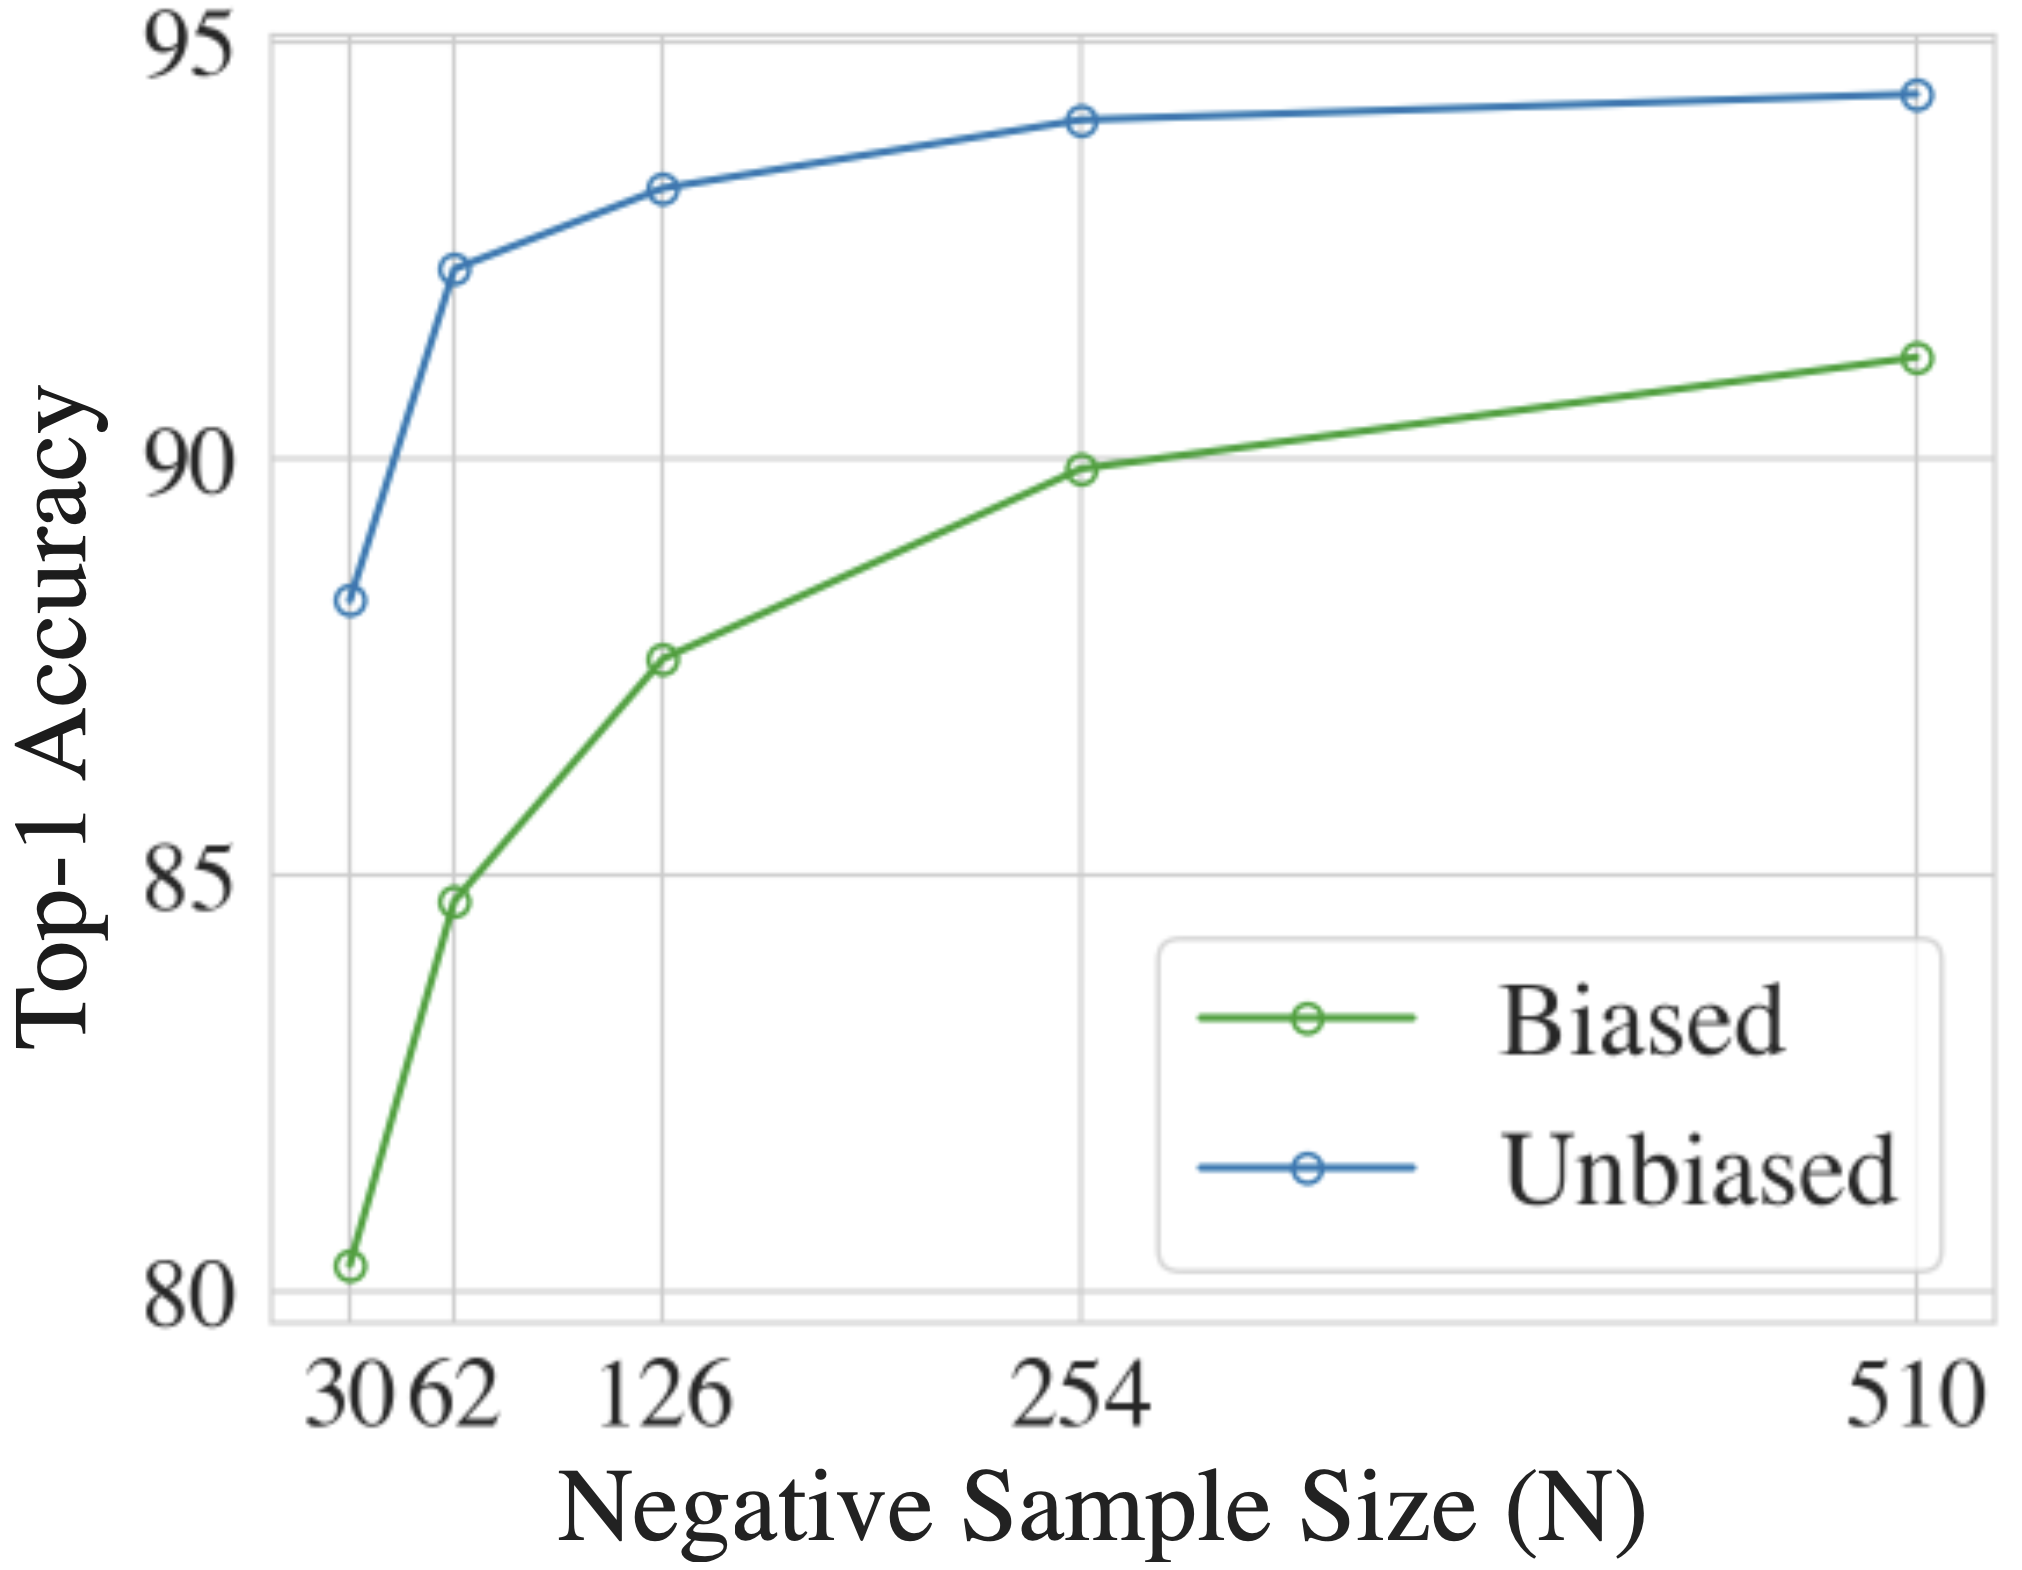
\includegraphics[width=5cm]{images/debiased_sampling_accuracy.png} }}%
    \caption{Visualization of sampling bias and its effect on the model's performance.}%
    \label{fig:sampling_bias}%
\end{figure}

\citeauthor{chuang_debiased_2020} assume a \ac{pu} learning scenario, 
where a positive sample and an unlabeled dataset $p(x)$ are available.
The positive distribution $p^+$ is mimicked by data augmentations.
The empirical estimation of the objective is given in 
\autoref{eq:debiasing_loss} from \citet{chuang_debiased_2020},
which is easier to compute than the original objective.
The negative samples $x^-$ are sampled from the data distribution $p(x)$.
However, the authors added a correction term for positive samples $x^+$.
The weighting factor $Q$ is used to balance the debiasing effect.

\begin{equation}
    \mathbb{E}_{x \sim p; x^+ \sim p^+}[{-\log{\frac{e^{f(x)^Tf(x^+)}}{e^{f(x)^Tf(x^+)}+ \frac{Q}{\tau^-}(\mathbb{E}_{x^- \sim p}[e^{f(x)^Tf(x^-)}]-\tau^+\mathbb{E}_{v \sim p^+}[e^{f(x)^Tf(v)}])}}}]
    \label{eq:debiasing_loss}
\end{equation}

% end

% ---- Bibliography ----

% \bibliographystyle{splncs04}
\bibliographystyle{unsrtnat}
\bibliography{references}



\begin{acronym}

    \acro{nn}[NN]{Neural Network}
    \acro{cl}[CL]{Contrastive Learning}
    \acro{pu}[PU]{Positive-Unlabeled}
    \acro{fn}[FN]{False Negative}
    \acro{tn}[TN]{True Negative}
    \acro{ssl}[SSL]{Self-Supervised Learning}
    \acro{clae}[CLAE]{Contrastive Learning with Adversarial Examples}
    \acro{fgsm}[FGSM]{Fast Gradient Sign Method}

\end{acronym}

\end{document}
